I am done with work at the employer for 2022. It was definitely an
experience. It was a great thing to have been able to do.

In the coming days I have plenty of things to do. The Christmas Eve
service was promoted in \emph{The} (Jefferson, Ohio) \emph{Gazette}
nicely. I did take a snapshot of the press release's insert.

\begin{figure}
\centering
\pandocbounded{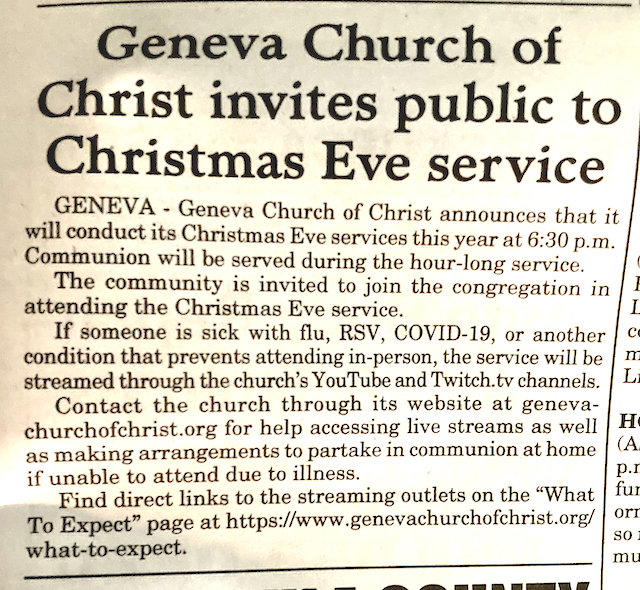
\includegraphics[keepaspectratio]{\%7B\%7Bsite.url\%7D\%7D/img/gcc-eve-service-announcement.jpg}}
\caption{Snapshot of the press release from Geneva Church of Christ}
\end{figure}

I'll be helming one aspect of tech services that night or another. I
don't think I have any speaking role that night. As to Christmas Day I
will be handling the communion meditation.

\href{https://developer.roku.com/docs/direct-publisher/overview.md}{Roku
Direct Publisher} is the next thing I need to fuss over. If I can get
that to work with items hosted on the
\href{https://archive.org/details/movies}{Internet Archive} then the
infrastructure behind \href{https://coyote.works/}{ELP TV} can be reset
to be a local video podcast channel. We already have the
\href{https://coyote.works/howtouse.html}{``how to subscribe''} language
posted for ELP TV. Having a Roku app on the one hand and using the
\href{https://web.archive.org/web/20221007010350/https://support.apple.com/en-ge/guide/tv/atvbb0659155/tvos}{Podcasts
app on Apple TV} would give fairly decent set-top box coverage for a
lower-budget television service. This is moving from being a blue skies
idea to something possibly in the realm of doable.

I suppose I need to look at
\href{https://rust-lang.github.io/mdBook/}{mdbook} to see what can be
done with it. Various bits of software need to be researched by me yet.
I additionally have to look at \href{https://cloud-init.io}{cloud-init}
to see if it can be used for making custom install images for ARM
devices. There may be other ways such as
\href{https://live-team.pages.debian.net/live-manual/html/live-manual/index.en.html}{live-build}
although live-build is possibly somewhat complex. Making a custom
loaded-up image of Xubuntu with my preferred set of installed packages
added is the goal in trying to build an ARM image so as to reduce wear
on an SD card.

Gears are shifting here. There are likely new adventures to come.
Undiscovered country awaits in the future.
